\documentclass[10pt,a4paper]{article}
\usepackage[utf8]{inputenc}
\usepackage{amsmath}
\usepackage{amsfonts}
\usepackage{amssymb}
\usepackage{graphicx}
\usepackage{times}
\usepackage{verbatim}
\usepackage{listings} 
\usepackage{graphicx}


\usepackage{ifpdf}
\ifpdf
\usepackage[breaklinks,colorlinks,linkcolor=black,citecolor=black,
            urlcolor=black]{hyperref}
\else
\usepackage{url}
\fi


\author{Mashruf Zaman Chowdhury}
\pagestyle{plain}
\usepackage[top=1in, bottom=1in, left=1in, right=1in]{geometry}


\usepackage{enumitem}
\setitemize{nolistsep,leftmargin=*}


\usepackage{listings}
\usepackage{color}

\definecolor{dkgreen}{rgb}{0,0.6,0}
\definecolor{gray}{rgb}{0.5,0.5,0.5}
\definecolor{mauve}{rgb}{0.58,0,0.82}

\lstset{frameround=ffff,
  language=bash,
  aboveskip=2mm,
  belowskip=2mm,
  showstringspaces=false,
  columns=flexible,
  basicstyle={\small\ttfamily},
  numbers=none,
  numberstyle=\tiny\color{blue},
  keywordstyle=\color{blue},
  commentstyle=\color{dkgreen},
  stringstyle=\color{blue},
  breaklines=true,
  breakatwhitespace=true,
  tabsize=3
}

\begin{document}
\title{Robotics Project: ROS-Turtlebot Motion Control $\&$ Navigation} \author{Yanik Porto \and Mashruf Zaman \and AK Assad} \date{\today}
\maketitle

\lstset{language=Python}% Set your language (you can change the language for each code-block optionally)

\tableofcontents

\newpage
\section[Part 1 - Motion Control]{Part 1 - Motion Control}

\subsection{Understanding the basics}

\begin{itemize}
\itemsep0em 
\item Nodes: A node is an executable that uses ROS to communicate with other nodes.
\item Messages: ROS data type used when subscribing or publishing to a topic.
\item Topics: Nodes can publish messages to a topic as well as subscribe to a topic to receive messages.
\item Master: Name service for ROS (i.e. helps nodes find each other)
\item rosout: ROS equivalent of stdout/stderr, This is always running as it collects and logs nodes' debugging output.
\item roscore: Master + rosout + parameter server %
(parameter server will be introduced later)
\end{itemize}

\subsection{Levels of Motion Control}
Controlling a mobile robot can be done at a number of levels and ROS provides methods for most of them.

\begin{center}
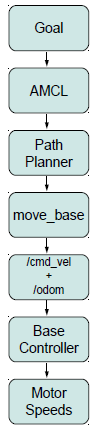
\includegraphics[width=0.2\textwidth]{images/motion_control.png}\\
\end{center}

\subsubsection{Motors, Wheels and Encoders}
Turtlebot uses \textbf{Encoders} to drive it's motors or wheels. Encoder registers certain number of ticks per revolution for a wheel. Knowing the diameter and distance between the wheels, from these ticks we can find distance traveled by the robot. To compute speed, these values are simply divided by the time interval between measurements.
This internal motion data is known as \fbox{odometry}. Due to Environmental and other errors this data is not generally accurate. We need to use other motion data sources to get better estimation.

\subsubsection{Motor Controllers and Drivers}
At the lowest level of motion control, a \textbf{driver }for the robot's motor controller turns the wheels at a desired speed, usually using internal units such as \textbf{encoder ticks per second} or a percentage of max speed.

\subsubsection{The ROS Base Controller}
At this level of abstraction, the desired speed of the robot is specified in real-world units such as meters and radians per second. It also commonly employs some \textbf{PID control }(Proportional Integral Derivative), which in layman terms generally does it's best to move the robot in the way we have requested. 

The driver and PID control are combined inside a single ROS node called \textbf{base controller}. 

The base controller node typically publishes odometry data on the \textbf{/odom }topic and listens for motion commands on the \textbf{/cmd\_vel} topic.

Also a transform from the \textbf{/odom} frame to the base frame—either \textbf{/base\_link} or /\textbf{base\_footprint (Turtlebot)} is done depending on the robot types.

Once we have our \textbf{base controller with a ROS interface} our programming can focus purely on the desired linear and angular velocities in real-world units.

\subsubsection{Frame-Base Motion using the move\_base ROS Package}
The \textbf{move\_base} package is a very sophisticated path planner and combines \textbf{odometry data} with both \textbf{local and global cost maps }when selecting a path for the robot to follow. We discuss more about \textbf{move\_base} in Navigating with Path Planning section.

\subsubsection{SLAM using the gmapping and amcl ROS Packages}
At an even higher level, ROS enables our robot to create a map of its environment using the SLAM gmapping package.

Once a map of the environment is available, ROS provides the amcl package (adaptive Monte Carlo localization) for automatically localizing the robot based on its current scan and odometry data.

\subsubsection{Semantic Goals}
Finally, at the highest level of abstraction, motion goals are specified semantically such as "go to the kitchen and bring me a beer", or simply, "bring me a beer". These are generally segmented into smaller tasks and passed to lower levels.

\subsection{Setting up the Network}

The primary requirement for getting your TurtleBot running is connecting to a network so that we can operate it remotely. After both TurtleBot and Workstation is connected to a network, it is time to set ROS\_MASTER\_URI and ROS\_HOSTNAME. The ROS\_MASTER\_URI tells the rest of the nodes at which address they can find the ROS master.\\

Here we setup the TurtleBot netbook as a ROS Master and our Workstation as a ROS node. Before this is done, we need to determine the IP address of your TurtleBot netbook and Workstation. This can be found by typing ``ifconfig'' in a terminal. Our IP address are found under wlan0, and it's the numbers proceeding ``inet addr:''.

\begin{lstlisting}[frame=single] 
> echo export ROS_MASTER_URI=http://IP_OF_TURTLEBOT:11311 >> ~/.bashrc
> echo export ROS_HOSTNAME=IP_OF_WORKSTATION >> ~/.bashrc
\end{lstlisting}
For ROS to operate you need to have an instance of roscore running on the master. We type the following command in the master:

\begin{lstlisting}[frame=single] 
$ roscore
\end{lstlisting}
These commands will add the export lines to the system bashrc file so they will run on every new terminal instance. This could also be done using an editor with command like $gedit \sim/.bashrc$ and saving the IP addresses there.

\subsection{Testing with the fake and the real Turtlebot}
The programs can be tested both in a simulated environment and in the real robot. However, when testing the real robot using the current configuration of the kobuki base in the turtlebot, it is necessary to remap the topic $\textbf{/mobile\_base/commands/velocity}$ to $/\textbf{cmd\_vel}$. In order do this, a launch file is created to remap this topic, in fact in every launch file we changed the topic like this.

\subsection{Goal 1 Basic Motion of Mobile Base}

We can do this in two way - from command prompt or by using a node. We see both way - 
\subsubsection{From command prompt}
ROS uses the \textbf{Twist message} type for publishing motion commands to be used by the base controller. While we could use almost any name for a topic, it is usually called \textbf{/cmd\_vel} which is short for "command velocities". The base controller node subscribes to the \textbf{/cmd\_vel} topic and translates \textbf{Twist messages} into motor signals that actually turn the wheels.

We can see the components of a \textbf{Twist message} using the following command:\\\\
\fbox{\$rosmsg show geometry\_msgs/Twist}\\

The Twist message is composed of two sub-messages with type Vector3, one for the x, y and z linear velocity components and another for the x, y and z angular velocity components. Linear velocities are specified in \underline{meters per second} and angular velocities are given in \underline{radians per second}.\\

By the following command we say the robot to go in linear direction 0.15 meter/s and at the same time change angular direction (z axis) clockwise 0.4 rad/s. For example if we wanted to rotate a full revolution per 2 second we had to use 3.14 as z value.
\begin{lstlisting}[frame=single] 
$roslaunch turtlebot_le2i remap_rplidar_minimal.launch (Bring up turtlebot)
$rostopic pub -r 10 /cmd_vel geometry_msgs/Twist '{linear: {x: 0.15, y: 0, z: 0}, angular: {x: 0, y: 0, z: -0.4}}'
\end{lstlisting}
We initialize the launch file and Publish \textbf{geometry\_msgs/Twist} message in the \textbf{/cmd\_vel} topic using ``rostopic'' command. Here \textbf{-r} is an option by which we say to do 10 repetitions.

\subsubsection{By using a node}
To do this we run a python script from ROS-by-Example (rbx1) packages. At first we go to our \textbf{/ros\_workspace} directory and clone the repo and make the package using the following commands:

\begin{lstlisting}[frame=single] 
$git clone https://github.com/pirobot/rbx1.git
$cd rbx1
$rosmake
$rospack profile
\end{lstlisting}

From command prompt we just use one command at a time. But we want to do some sequential tasks, so it is better to give commands again and again then to put them in a source code file or node. \\
We use timed Twist commands to move the robot forward a certain distance, rotate 180 degrees, then move forward again for the same time and at the same speed where it will hopefully end up where it started. Finally, we will rotate the robot 180 degrees one more time to match the original orientation.\\

\textbf{Algorithm 1: Time and Speed based out and back}
\begin{lstlisting}[frame=single]
rate = 50
goal_distance = 1.0 m
linear_speed = 0.2m/s
linear_duration = goal_distance / linear_speed;

angular_speed = 1.0
goal_angle = pi
angular_duration = goal_angle / angular_speed;

A: Repeat step 1 to 6 twice

	1. ticks = linear_duration / rate
	2. while(t < ticks)
		robot will walk 1 meter straight
	3. robot will sleep 1 cycle
	
	4. ticks = goal_angle * rate
	5. while(t<ticks)
		robot rotates 180*
	6. robot will sleep 1 cycle
	
B: Program Terminates
\end{lstlisting}

This is a \textbf{Time and Speed} based approximation, which we shall see will not be as accurate as expected. Here are the code segments to do it:

We ssh into the turtlebot and run the follwing scripts
on Turtlebot:
\begin{lstlisting}[frame=single] 
$roslaunch turtlebot_le2i remap_rplidar_minimal.launch (Bring up turtlebot)
\end{lstlisting}
We are going to configure to subscribe to combined odometry data (encoders + gyro) 
rather than \textbf{/odom} topic which only shows the encoder data. Hence we run this script
\begin{lstlisting}[frame=single] 
$roslaunch rbx1_bringup odom_ekf.launch
\end{lstlisting}

\textbf{On Workstation:}\\
run \textbf{rviz} to see the combined odometry data. This is displaying the combined odometry data on the \textbf{/odom\_ekf} topic rather than just the wheel encoder data published on the \textbf{/odom} topic.
\begin{lstlisting}[frame=single] 
$rosrun rviz rviz -d `rospack find rbx1_nav`/nav_ekf.rviz
\end{lstlisting}
finally we run the python script to do the previously defined task 
\begin{lstlisting}[frame=single] 
$rosrun rbx1_nav timed_out_and_back.py
\end{lstlisting}

Now we can see from rviz is that, the robot didn't do actually what is supposed to do
because of environmental constraint. It messed up but we have unfairly handicapped it 
by not using the odometry data in our script. Our script based only on time and speed. 
While the odometry data will not match the real motion exactly, 
it should give us a better result if we use it. We shall see it in the next step

\subsection{Goal 2 = Advanced Motion of Mobile Base}
let's assume that we have some data from the laser in the form of distances from the laser's center point. In other words, we have some data in the \textbf{``base\_laser"} coordinate frame. Now suppose we want to take this data and use it to help the mobile base avoid obstacles in the world. To do this successfully, we need a way of transforming the laser scan we've received from the \textbf{``base\_laser"} frame to the \textbf{``base\_link"} frame. In essence, we need to define a relationship between the \textbf{``base\_laser"} and \textbf{``base\_link"} coordinate frames.\\

\begin{center}
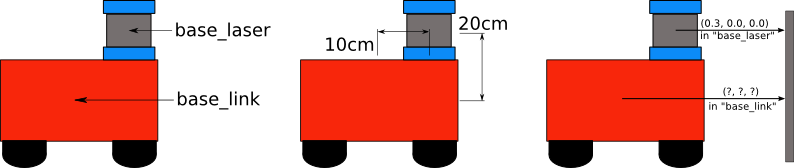
\includegraphics[width=\textwidth]{images/simple_robot.png}\\
\end{center}

Such is the case for the turtlebot Odometry data we use to move the robot.
While the \textbf{/base\_link} frame corresponds to a real physical part of Controlling a Mobile Base robot, the \textbf{/odom} frame is defined by the translations and rotations encapsulated in the odometry data. These transformations move the robot relative to the \textbf{/odom} frame.
In ROS if we see the \textbf{nav\_msgs/Odometry} message structure, \textbf{/odom }is used as the parent frame and \textbf{/base\_footprint} (for turtlebot) as the \textbf{child\_frame\_id}. The transformation between these two frames, is with the help of tf library.

Rather than guessing distances and angles based on time and speed, our next script will monitor the robot's position and orientation as reported by the transformation between the \textbf{/odom }and \textbf{/base\_footprint} frames.


\textbf{Algorithm 2: ODOMETRY based out and back}
\begin{lstlisting}[frame=single]
rate = 50
goal_distance = 1.0 m
linear_speed = 0.2m/s
linear_duration = goal_distance / linear_speed;

angular_speed = 1.0
goal_angle = pi
angular_duration = goal_angle / angular_speed;

A: Repeat step 1 to 6 twice

	1. get initial position
	2. while distance < goal_distance
		robot will go at a speed set by linear_speed
		sleep 1 cycle
		get new linear position from ODOMETRY
		calculate new distance from new position and  old position
	3. stop the robot
		Set last_angle = rotation
			turn_angle = 0
	4. while (turn_angle < goal_angle)
		start rotating
		sleep 1 cycle
		get new rotation position from ODOMETRY
		delta_angle = (rotation - last_angle)
		turn_angle += delta_angle
		last_angle = rotation	
	5. stop the robot 1 cycle before next run
	
B: Program Terminates
\end{lstlisting}


We ssh into the turtlebot and run the follwing scripts
on Turtlebot:
\begin{lstlisting}[frame=single] 
$roslaunch turtlebot_le2i remap_rplidar_minimal.launch (Bring up turtlebot)
\end{lstlisting}
We are going to configure to subscribe to combined odometry data (encoders + gyro) 
rather than \textbf{/odom }topic which only shows the encoder data. Hence we run this script
\begin{lstlisting}[frame=single] 
$roslaunch rbx1_bringup odom_ekf.launch
\end{lstlisting}

On Workstation:
run rviz to see the combined odometry data
This is displaying the combined odometry data on the \textbf{/odom\_ekf} 
topic rather than just the wheel encoder data published on the \textbf{/odom} topic.
\begin{lstlisting}[frame=single] 
$rosrun rviz rviz -d `rospack find rbx1_nav`/nav_ekf.rviz
\end{lstlisting}

finally we run the python script to do the previously defined task 
\begin{lstlisting}[frame=single] 
$rosrun rbx1_nav odom_out_and_back.py
\end{lstlisting}

Using odometry the results improves significantly from the timed out-and-back case, because still accuracy and reliability of this process depends on the robot's internal sensors, the accuracy of the calibration procedure, and environmental conditions.
Since the robot is performing a very simple task, the navigation error is slight, and it is more evident after performing the task successively several times.

\begin{center}
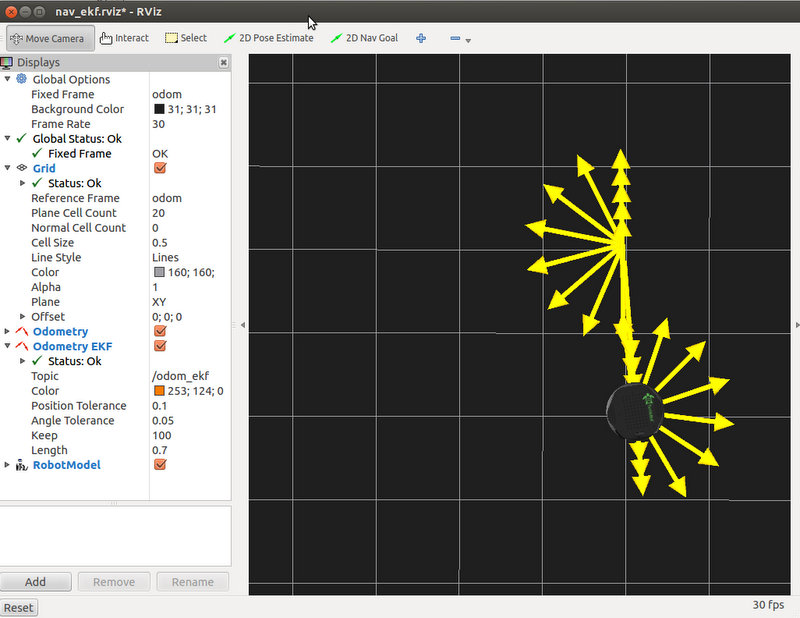
\includegraphics[width=\textwidth]{images/odom_out_and_back.jpg}\\
\end{center}

\subsubsection{Dead Reckoning}
Even small amount of error in the robot odometry data accumulates over time. Hence a robot navigating only using internal motion data and without any reference to external landmarks will grow on it's mistakes and eventually be completely lost. This is knows as Dead Reckoning. \\
We can improve this for our turtlebot using map and SLAM.

\subsection{Goal 3 = Navigating a Square using Twist+Odometry}
In a similar way to the previous Goal, in Goal 3 the robot navigates through a square path, using both Twist and Odometry messages.

However, this time we will attempt to move the robot in a square by setting four waypoints, one at each corner. At the end of the run, we can see that the errors accumulated in odometry are more visible:

\begin{center}
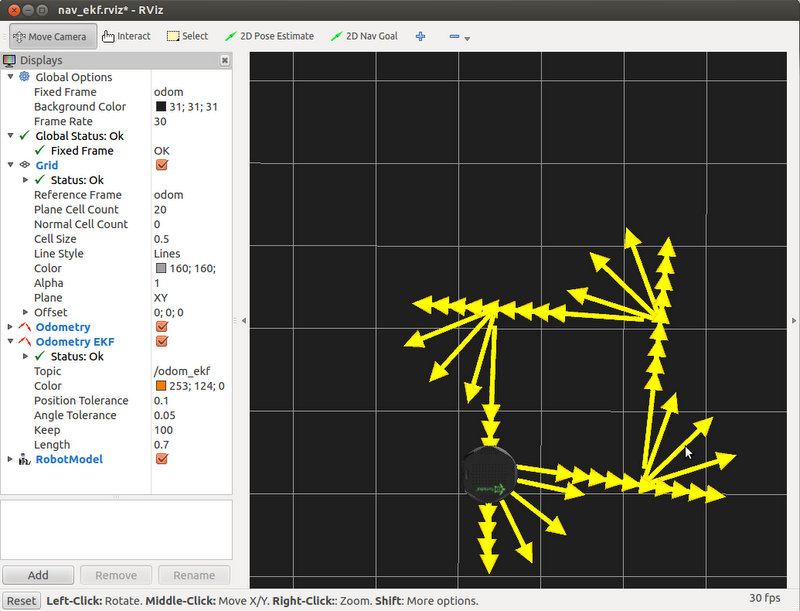
\includegraphics[width=\textwidth]{images/square_py.jpg}\\
\end{center}

\subsection{Goal 4 = Navigation with Path Planning move\_base}
ROS provides the move\_base package that allows us to specify a target position and orientation of the robot with respect to some frame of reference.

Following figure summarizes how the move\_base path planner works. On the bottom left of figure is a base controller node for low level motion control. on the top right is the map server which provides a map of environment.

\begin{center}
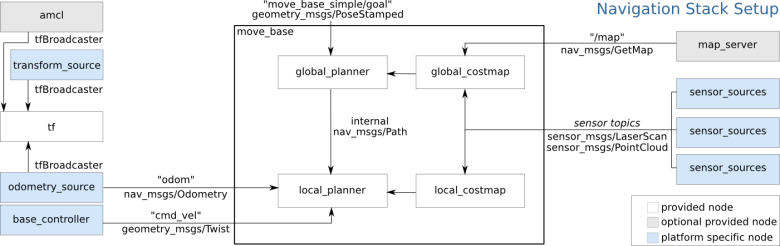
\includegraphics[width=\textwidth]{images/overview_small.png}
\end{center}

\begin{center}
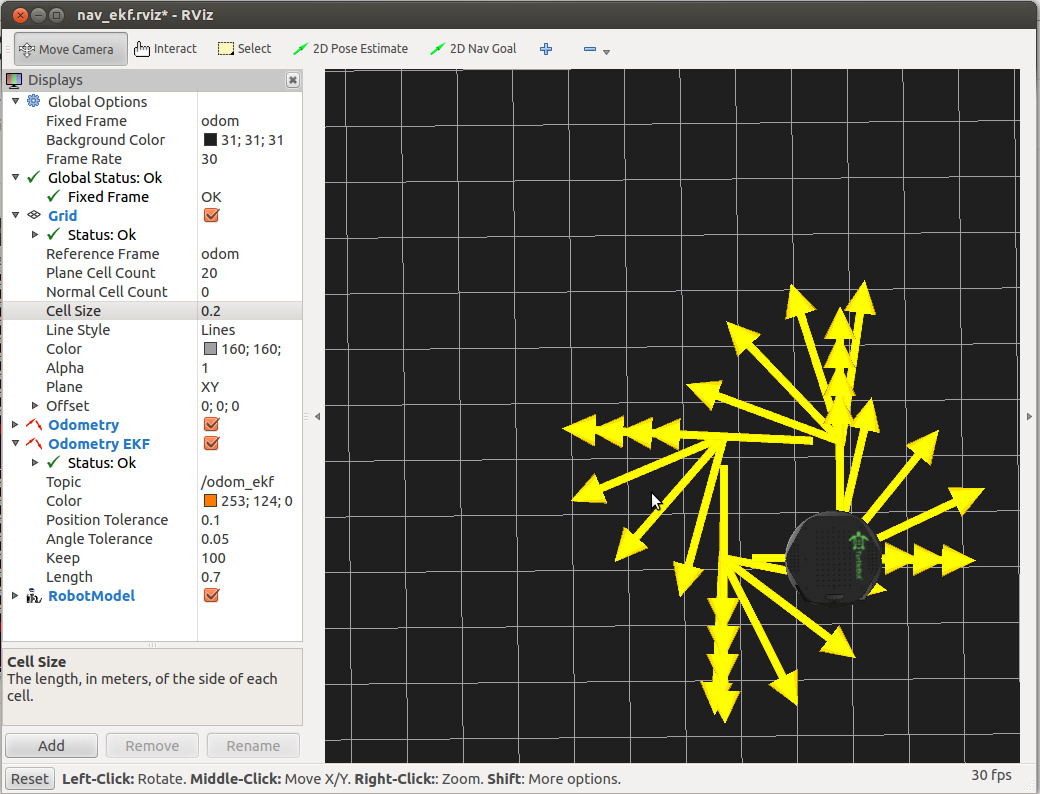
\includegraphics[width=\textwidth]{images/move_base_square.jpg}\\
\end{center}

\textbf{A video of this movement can be seen here:}\\
\fbox{\url{https://www.youtube.com/watch?v=5e61iTaRLl0}}

\section{Part 2 - Planar Laser RangeFinder}

\subsection{RP-LIDAR}

\begin{center}
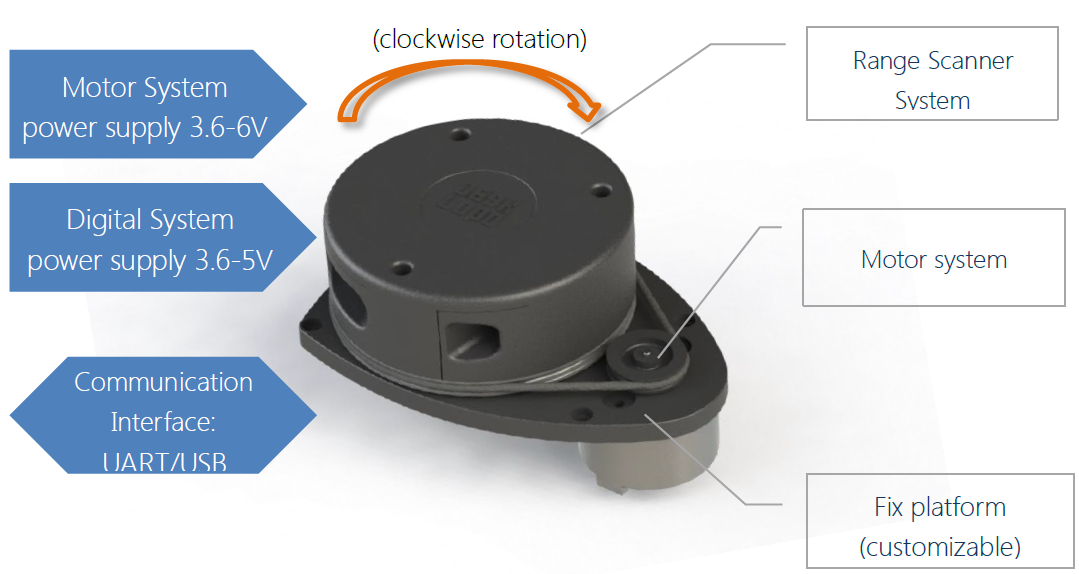
\includegraphics[scale=0.4]{images/lidarParts.png}\\
\textit{The different RP-LIDAR's parts}
\end{center}

RP-LIDAR is a low-cost \textbf{360 degree} 2D Laser Scanner (LIDAR) system.\\
It can perform scanning with a frequency of\textbf{ 5.5Hz} when sampling 360 points within \textbf{6 meter range}. \\

RP-LIDAR is based on \textbf{laser triangulation ranging principle} :\\
It emits modulated infrared laser signal and the laser signal is then reflected by the object to be detected. The returning signal is sampled by vision acquisition system in RP-LIDAR and the DSP embedded in RP-LIDAR start processing the sample data, output distance value and angle value between object and RP-LIDAR through communication interface.\\

\begin{center}
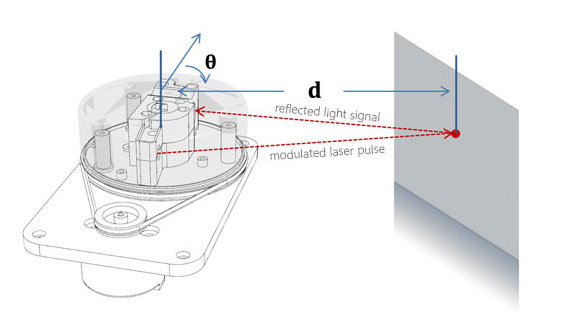
\includegraphics[scale=0.6]{images/robopeak-sensor.jpg}\\
\textit{Graphical representation of laser triangulation}
\end{center}

The system can measure distance data in more than 2000 times' per second and with high resolution distance output ($<$1\% of the distance) :\\

\begin{center}
\begin{tabular}{|l|c|l|}
\hline
Data Type & Unit & Description\\
\hline
Distance & mm & Current measured distance value\\
%\hline
Heading & degree & Current heading angle of the measurement \\
%\hline
Quality & level & Quality of the measurement\\
%\hline
Start Flag & 	(Boolean) & Flag of a new scan\\
\hline
\end{tabular}\\

\textit{Output data given by RP-LIDAR}
\end{center}

These data will be used in order to scan a map and to move the turtlebot in function of this map and the points detected. 

\begin{center}
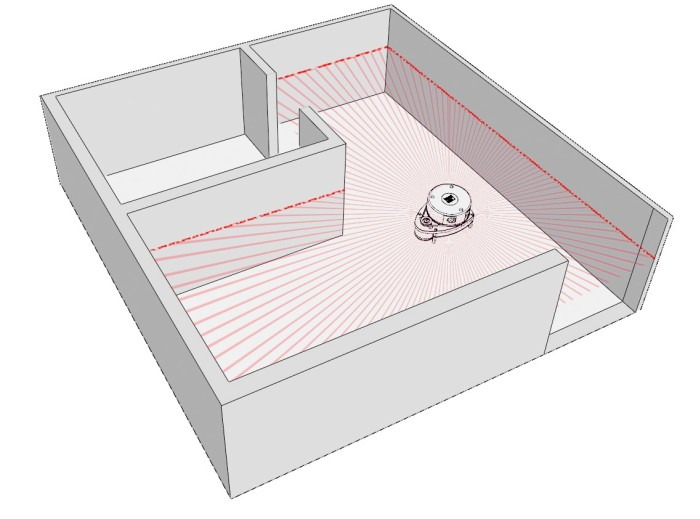
\includegraphics[scale=0.5]{images/RPLIDAR_room.jpg}\\
\textit{Example of scanned map using RP-LIDAR}
\end{center}

\subsection{Integration on Turtlebot2}

\subsubsection{rplidar$\_$ros package}
The package \textbf{"rplidar\_ros"} needs to be added to integrate the RP-LIDAR to ROS. 
As this package is only available in \textbf{Ros Hydro}, this ROS distribution will be used (the buildsystem \textbf{"Catkin"} is also required).\\
Once it has been done, the most important informations we want are located in the rplidar node (\textbf{rplidarNode}).\\
The \textbf{rplidarNode} is a driver for RP-LIDAR which reads RP-LIDAR raw scan result using RPLIDAR's SDK and convert the informations to messages in the topic \textbf{sensor\_msgs/LaserScan}.\\

This node is created with the help of the \textbf{\underline{rplidar.launch}} file, located in the \textbf{"rplidar\_ros"} package.
All the parameters needed for the Lidar are stated in this file : \\

\begin{lstlisting}[frame=single] 
<launch>
  <node name="rplidarNode"          pkg="rplidar_ros"  type="rplidarNode" output="screen">
  <param name="serial_port"         type="string" value="/dev/ttyUSB1"/>  
  <param name="serial_baudrate"     type="int"    value="115200"/>
  <param name="frame_id"            type="string" value="base_laser_link"/>
  <param name="inverted"            type="bool"   value="false"/>
  <param name="angle_compensate"    type="bool"   value="true"/>
  </node>
</launch>
\end{lstlisting}


\subsubsection{turtlebot$\_$le2i package}


Then it is necessary to create a new package where the position of the Lidar on the turtlebot, compared with the "[parent]" is given (which in our case is the \textbf{plate\_top\_link}). This will be used by the  $\textbf{tf}$ node, to compute the laser position compared to the base. \\
In our case, this package is named \textbf{"turtlebot\_le2i"}. It contains a bringup launch file called \textbf{rplidar\_minimal.launch} which launch the simple bringup \textbf{minimal.launch}, the \textbf{rplidar.launch} and also some .xml files. \\
In these files, one is the \textbf{\underline{rplidar.urdf.xacro}}.
It contains all about the RP-LIDAR position : the origin, the box size, ...  Here is a part of this file : 

\begin{lstlisting}[frame=single] 
	<xacro:macro name="sensor_rplidar" params="parent">
  	<joint name="laser" type="fixed">
		<origin xyz="0.180 0.00 0.040" rpy="0 3.14159265 0" />
		<parent link="${parent}" />
		<child link="base_laser_link" />
	</joint>

	<link name="base_laser_link">
		<visual>
			<geometry>
				<box size="0.00 0.05 0.06" />
			</geometry>
			<material name="Green" />
		</visual>
		<inertial>
			<mass value="0.000001" />
			<origin xyz="0 0 0" />
			<inertia ixx="0.0001" ixy="0.0" ixz="0.0"
			iyy="0.0001" iyz="0.0" izz="0.0001" />
		</inertial>
	</link>
	</xacro:macro>
\end{lstlisting}
\underline{Note} : Xacro is an XML macro language, used to construct shorter and more readable XML files.

\subsubsection{base$\_$laser$\_$link} 
\begin{center}
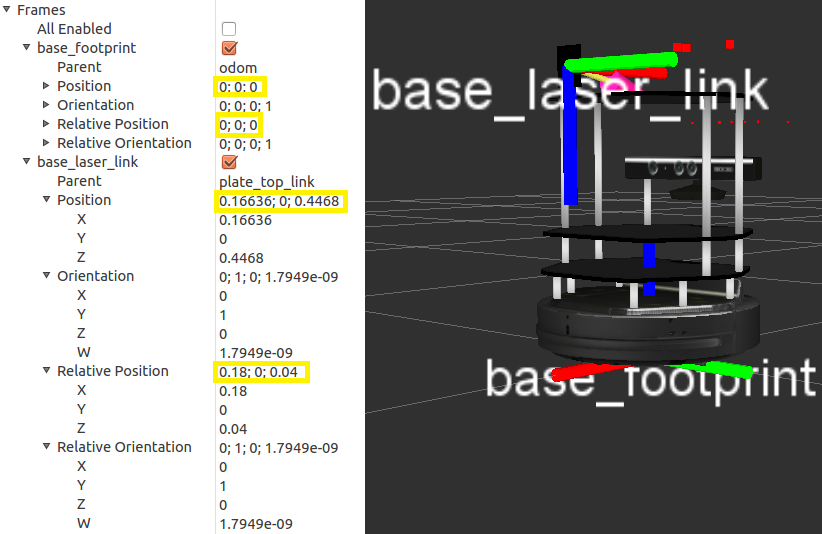
\includegraphics[width=\textwidth]{images/tf_coordinates_small.png}\\
\end{center}

You can see in the \textbf{"Relative Position"}, the values are the same as the coordinates stated in the .urdf (cf. \textit{Configure Ros}).\\
There is also the computed \textbf{"Position"} from the base to the lidar, thanks to the \textbf{tf} node taking into account the relative position from the \textbf{plate\_top\_link}, which has also a relative position compared with his parent and so on until the\textbf{base\_footprint}. \\

\subsubsection{Displaying the data}
To extract the data from the RP-LIDAR :\\
bringup the turtlebot, \\
then start a rplidar node and run \textbf{rplidar client process} to print the raw scan result :
\begin{lstlisting}[frame=single] 
$ roslaunch rplidar_ros rplidar.launch
$ rosrun rplidar_ros rplidarNodeClient
\end{lstlisting}

\begin{center}
%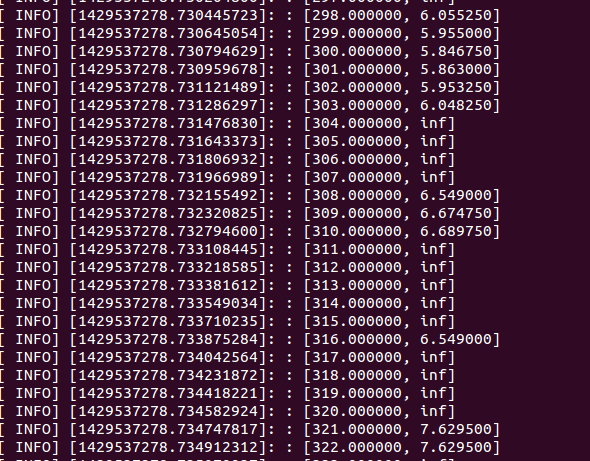
\includegraphics[width=0.5\textwidth]{images/rplidarInfo.png}\\
\end{center}

To see the data coming from the RP-LIDAR :\\
bringup the turtlebot, \\
then start a rplidar node and view the scan result in rviz:
\begin{lstlisting}[frame=single] 
$ roslaunch rplidar_ros view_rplidar.launch
\end{lstlisting}

\begin{center}
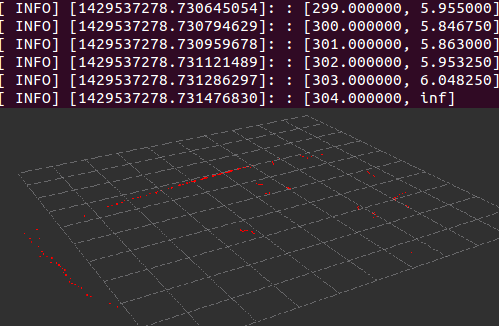
\includegraphics[width=\textwidth]{images/infos+view.png}\\
\end{center}

This scanner will be used here, for the application of general simultaneous localization and mapping (SLAM).

\section{Part 3 - Navigation $\&$ Localization}
\begin{tabbing}
\hspace{1cm}\=\hspace{1cm}\=\kill
Three essential ROS packages that make up the core of navigation stack:	\\
\> - gmapping for creating map from RPlidar laser scan data \\
\> - amcl for the localization using an existing map \\
\> - move\_base for moving the robot to a goal within given reference frame \\
\end{tabbing}

\begin{center}
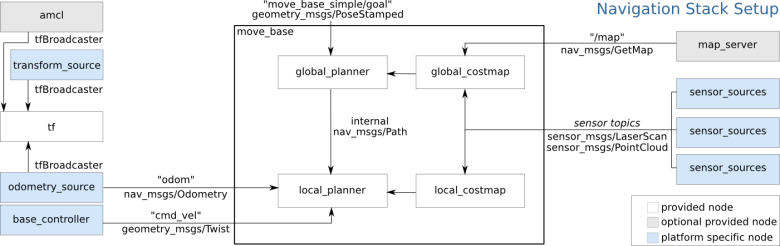
\includegraphics[width=\textwidth]{images/overview_small.png}
\end{center}

\subsection{Map Creation}

Although ROS based ROBOT’s can navigate in an unknown environment, it’s very ideal to create and use a map. In a known environment path planning/movement is much easier.  In the project, gmapping package was used to create a map with the help of teleop. \\

\subsubsection{Mapping}
	
Learning maps is one of the fundamental problems in mobile robotics. Maps allow robots to efficiently carry out their tasks, such as localization, path planning, activity planning, etc. There are different ways to represent the world space, such as: Grid maps, Geometric maps, Voronoi graphs \\

Occupancy Grid Map, Maps the environment as a grid of cells. Cell sizes typically range from 5 to 50 cm, each cell holds a probability value that the cell is occupied in the range [0,100], Unknown is indicated by -1, Usually unknown areas are areas that the robot sensors cannot detect (beyond obstacles)

\begin{center}

\includegraphics[width=0.3\textwidth]{images/arena1.png}\\
White pixels represent free cells \\
Black pixels represent occupied cells \\
Gray pixels are in unknown state \\
\end{center}

\subsubsection{Marking and Clearing}

The grid map is built using a process called \textbf{marking} and clearing. A marking operation inserts obstacle information into the map. A \textbf{clearing} operation removes obstacle information from the map. It consists of \textbf{raytracing} through a grid from the origin of the sensor outwards for each observation reported.

\subsubsection{SLAM}
\textbf{Simultaneous localization and mapping} (\textbf{SLAM}) is a technique used by robots to build up a map within an unknown environment while at the same time keeping track of their current location.

\subsubsection{Gmapping}
Gmapping (http://wiki.ros.org/gmapping) package provides laser-based SLAM as a ROS node called \textbf{slam\_gmapping}. It Uses the FastSLAM algorithm. It takes the laser scans and the odometry and builds a 2D occupancy grid map. It updates the map state while the robot moves.

\subsection{SLAM Map Building with TurtleBot}

In order to navigate and localization the turtlebot, first the map of the arena needs to be created. Turtlebot already got the essential updates in order to use gmapping package while it been used for the navigation purpose describe earlier.

Following steps been used to create and save the map of arena:\\
To launch the gmapping package\\
on the TurtleBot :
\begin{lstlisting}[frame=single] 
$ roslaunch turtlebot_le2i rplidar_minimal.launch
$ roslaunch rbx1_nav rplidar_gmapping_demo.launch
\end{lstlisting}

For launching rviz in order to view and save the map\\
on the Workstation :
\begin{lstlisting}[frame=single] 
$ roslaunch turtlebot_rviz_launchers view_navigation.launch
$ roslaunch turtlebot_teleop keyboard_teleop.launch
\end{lstlisting}

\begin{center}
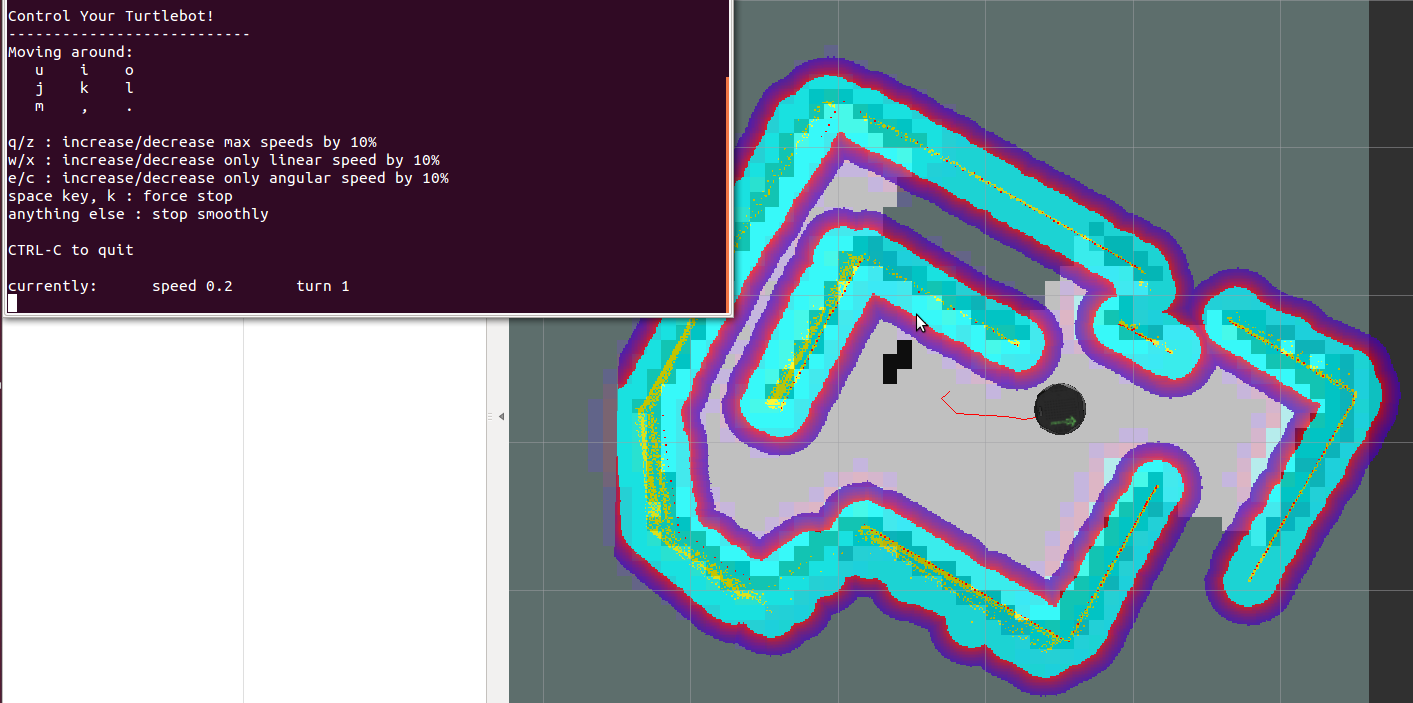
\includegraphics[width=\textwidth]{images/BuildingMap+keyboard.png}
\end{center}

\subsubsection{Saving Map}

The robot needed to drive around using telop keyboard slowly to get the entire arena. This process is used few times to circle the arena in order to record better map. \textbf{map\_server} package is used by ROS to load and save maps. \\

- Save the map to file:
\begin{lstlisting}[frame=single] 
$ rosrun map_server map_saver -f /tmp/my_map
\end{lstlisting}

\begin{tabbing}
\hspace{1cm}\=\hspace{1cm}\=\kill
map\_saver generates the following files in the directory:\\
\> \textbf{my\_map.pgm} – the map itself \\
\> \textbf{my\_map.yaml} – the map’s metadata \\
\end{tabbing}

\begin{center}
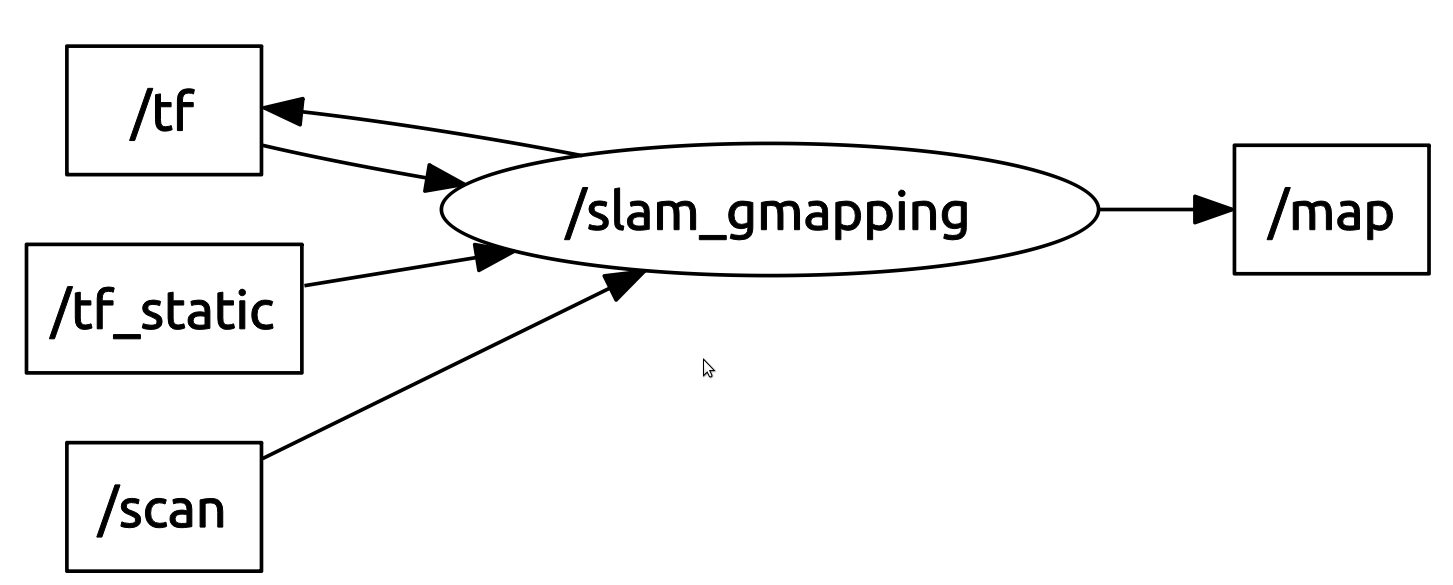
\includegraphics[width=0.8\textwidth]{images/nodes.png}
\end{center}

\begin{tabbing}
\hspace{1cm}\=\hspace{1cm}\=\kill
Some important fields:\\
\>  – \textbf{resolution:} Resolution of the map, meters / pixel \\
\>  – \textbf{origin:} The 2-D pose of the lower-left pixel in the map as (x, y, yaw) \\
\>  – \textbf{occupied\_thresh:} Pixels with occupancy probability greater than this threshold are considered completely occupied. \\
\> – \textbf{free\_thresh:} Pixels with occupancy probability less than this threshold are considered completely free. \\
\end{tabbing}

\subsection{Localization}

Localization is the problem of estimating the pose of the robot relative to a map. Localization is not terribly sensitive to the exact placement of objects so it can handle small changes to the locations of objects. ROS uses the amcl package for localization. Before using the navigation, it’s important to understand how amcl pacakage works. 

\subsection{Amcl}
amcl is a probabilistic localization system for a robot moving in 2D. It implements the adaptive (or KLD-sampling) Monte Carlo localization approach, which uses a particle filter to track the pose of a robot against a known map. amcl takes in a laser-based map, laser scans, and transform messages, and outputs pose estimates. On startup, amcl initializes its particle filter according to the parameters provided. As defaults, if no parameters are set, the initial filter state will be a moderately sized particle cloud centered about (0,0,0).

\begin{tabbing}
\hspace{1cm}\=\hspace{1cm}\=\kill
Subscribed topics:\\
\> - \textbf{scan} – Laser scans\\
\> - \textbf{tf} – Transforms\\
\> - \textbf{initialpose} – Mean and covariance with which to (re-) initialize the particle filter \\
\> - \textbf{map} – the map used for laser-based localization \\

Published topics:\\
\> - \textbf{amcl\_pose} – Robot's estimated pose in the map, with covariance\\
\> - \textbf{Particlecloud} – The set of pose estimates being maintained by the filter\\
\end{tabbing}

\begin{center}
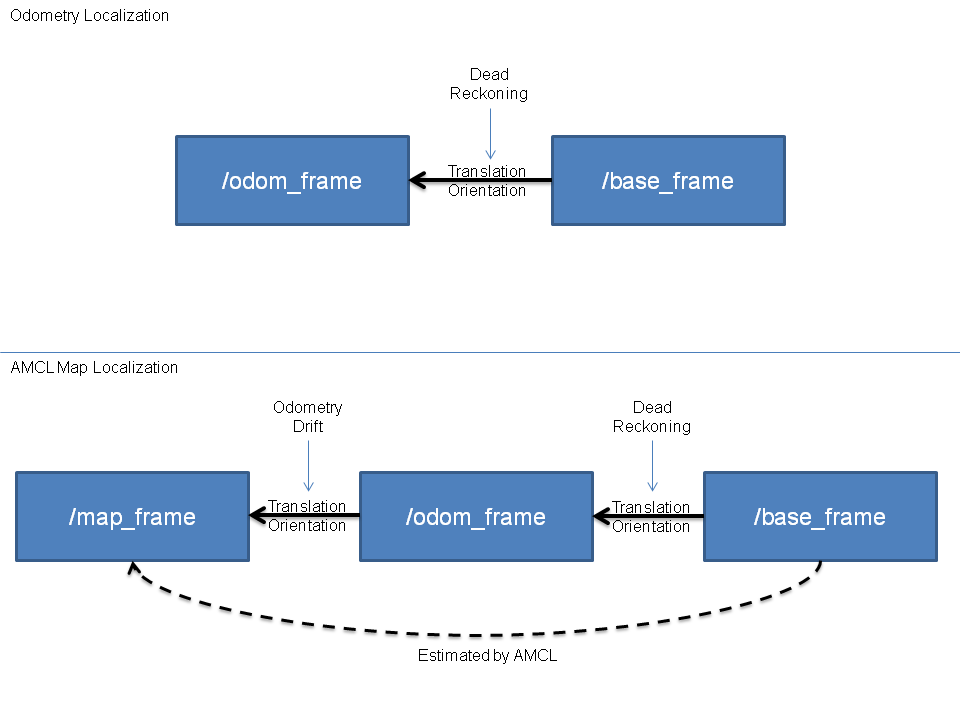
\includegraphics[width=0.8\textwidth]{images/amcl_localization.png}\\
\textit{The difference between odometry based localization and AMCL map localization}
\end{center}

\subsection{Navigation and localization using a map and amcl}

\begin{tabbing}
\hspace{1cm}\=\hspace{1cm}\=\kill
Navigating a robot in a map is done simply using amcl, existing map and Rviz. To run the navigation stack with amcl,  the following nodes needs to start: \\
\> -\textbf{ map\_server }– for loading the map\\
\> - \textbf{amcl} – for the localization system\\
\> - \textbf{move\_base} – manages the navigation stack\\
\end{tabbing}

Following steps, been used to run navigation \\
on the turtlebot netbook:
\begin{lstlisting}[frame=single]
$ roslaunch turtlebot_le2i remap_rplidar_minimal.launch
$ roslaunch rbx1_nav tb_demo_amcl.launch map:=arena.yaml
\end{lstlisting}

on the workstation : 
\begin{lstlisting}[frame=single]
$ roslaunch turtlebot_rviz_launchers view_navigation.launch
\end{lstlisting}

\subsubsection{Point and click navigation using Rviz}
After amcl bring up, the initial pose of the turtlebot is to be set, because amcl can’t do its own. To set the initial pose, just need to click on the “2D Pose Estimate” button in rviz. Then click on the point in the map where the robot is located. While holding down the mouse button, a large green arrow appears. The mouse then moved to orient the arrow to match the orientation of the robot, and then released. With the robots initial position set, it’s now possible to use the “2D Nav Goal” button in rviz to navigate goals of the turtlebot at different locations in the map of arena.\\

\subsubsection{Path Planning}
Path planning is based on WHERE am I and HOW to go there technique. To move from position A to position B turtlebot needs to know its initial position and path finding algorithm to reach its destination. ‘2D pose estimate’ uses the amcl package to set turtlebot position in the map. Path planning uses \textbf{Global plan} and \textbf{Local plan} to reach the goal. To understand the navigation it is very important to understand how both plan combined in order to reach the goal. \\

At the first try, the turtlebot was not able to reach its destination due to a L shape obstacle in the middle, the turtlebot continuously stacked and collide into the edge of the wall. After investigation, it is discovered that robots inflation is the factor in order to run the turtlebot smoothly in the arena. In order to fix the issues, it is very important to go through all the files contained by move\_base package. Using the values of local cost map, global cost map and the robot footprint, 2D\_Nav\_Goal determines the path and distance in order to reach the goal. \\

\subsubsection{Move\_base package}

The move\_base package provides an implementation of an action that, given a goal in the world, will attempt to reach it with a mobile base. The move\_base node links together a global and local planner to accomplish its global navigation task. It supports any global planner adhering to the \textbf{nav\_core::BaseGlobalPlanner} interface specified in the nav\_core package and any local planner adhering to the \textbf{nav\_core::BaseLocalPlanner} interface specified in the nav\_corepackage. The move\_base node also maintains two costmaps, one for the global planner, and one for a local planner that are used to accomplish navigation tasks.\\

Move\_base nodes requires four configuration files before it can run. These files defines a number of parameters related to the cost of running into obstacle, the radius of the robot, how fast the robot moves and how far the path planner should looks. \\

The four configuration files can be found in the \textbf{config} subdirectory of the \textbf{rbx1\_nav} package and are called: \\

base\_local\_planner\_params.yaml
\begin{lstlisting}[frame=single]
FILES
\end{lstlisting}
costmap\_common\_params.yaml
\begin{lstlisting}[frame=single]
FILES
\end{lstlisting}

global\_costmap\_params.yaml
\begin{lstlisting}[frame=single]
FILES
\end{lstlisting}

local\_costmap\_params.yaml 
\begin{lstlisting}[frame=single]
FILES
\end{lstlisting}

\subsubsection{Cost Map}

Cost map is a data structure that represents places that are safe for the robot to be in a grid of cell. It is based on the occupancy grid map of the environment and user specified inflation radius. There are two types of costmaps in ROS: Global costmap is used for global navigation and Local costmap is used for local navigation.

\underline{\textbf{Cost Map Value :}}\\

\begin{tabbing}
\hspace{1cm}\=\hspace{1cm}\=\kill
Each cell in the costmap has an integer value in the range [0, 255].There are 5 special symbols for cost values:\\
\> - \textbf{NO\_INFORMATION} (255) - Reserved for cells where not enough information is sufficiently known\\
\> - \textbf{LETHAL\_OBSTACLE} (254) - Indicates a collision causing obstacle was sensed in this cell\\
\> - \textbf{INSCRIBED\_INFLATED\_OBSTACLE} (253) - Indicates no obstacle, but moving the center of the robot\\ to this location will result in a collision\\
\> - \textbf{POSSIBLY CIRCUMSCRIBED} (128-252) – If the robot center lies in that location, then it depends\\ on the orientation of the robot whether it collides with an obstacle or not \\
\> - \textbf{FREE\_SPACE} (0) - Cells where there are no obstacles and the moving the center of the robot to this\\ position will not result in a collision\\
\end{tabbing}

\begin{center}
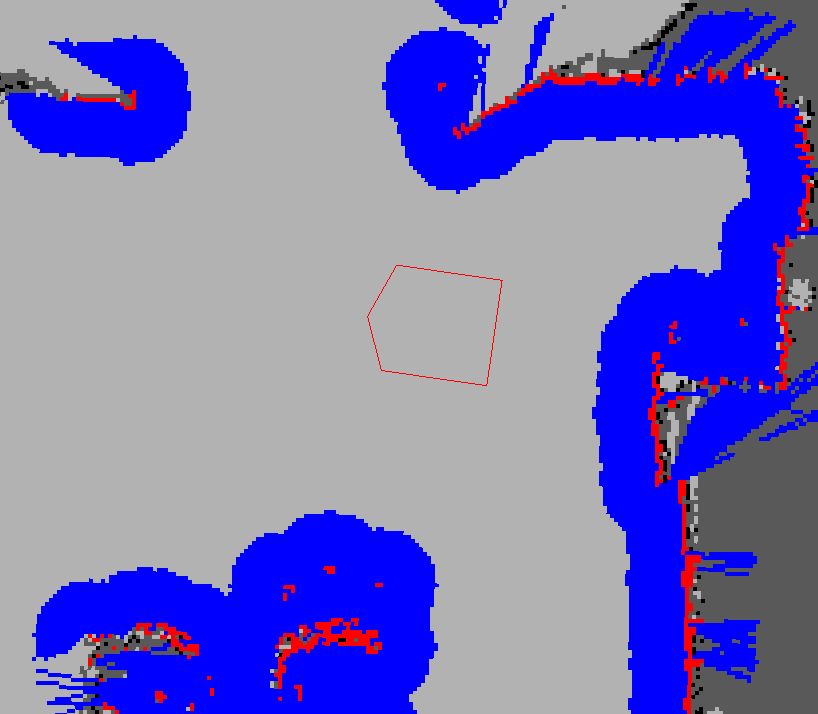
\includegraphics[width=0.5\textwidth]{images/costmap.png}\\
\textit{Example of cost map ros.wiki} \\
\end{center}


\underline{\textbf{Inflation Function :}}\\
Inflation is the process of propagating cost values out from occupied cells that decrease with distance. A brief explanation of inflation is given below:\\

\begin{center}
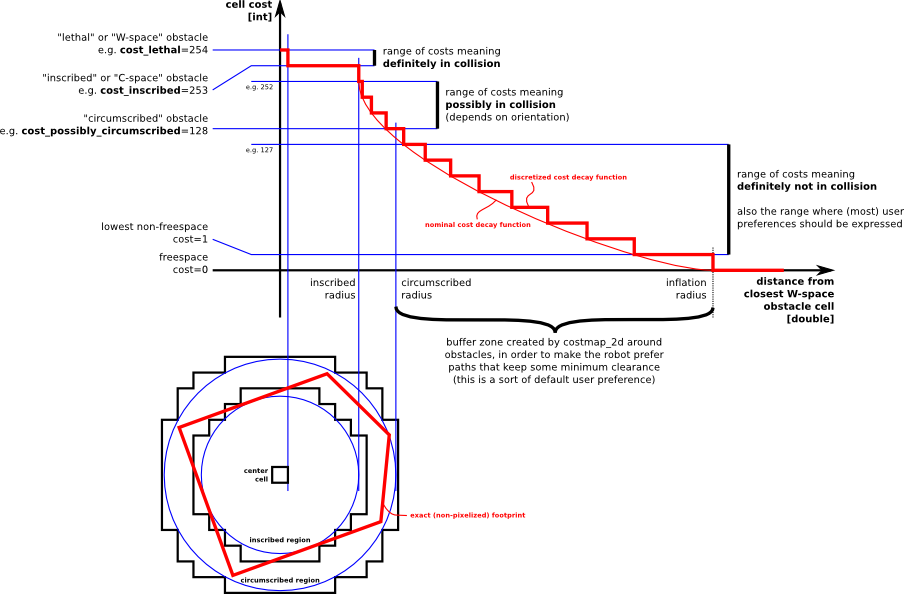
\includegraphics[width=0.7\textwidth]{images/inflation.png}\\
\end{center}

\subsubsection{Global Planner}

Map + Costs = Global Cost Map \\
Global Cost Map + Start + Target = Global Plan (way points)

\subsubsection{Local Planner}

Global map is static and using only global map can create problems especially when dynamic objects or obstacles are placed in the map. 
For the local path planner cost is calculated as below:
Cost = path\_distance\_bias * (distance to path from the endpoint of the trajectory in map cells or meters depending on the meter\_scoring parameter) + goal\_distance\_bias * (distance to local goal from the endpoint of the trajectory in map cells or meters depending on the meter\_scoring parameter) + occdist\_scale * (maximum obstacle cost along the trajectory in obstacle cost (0-254)).\\

\underline{\textbf{Navigation in action :}}\\
The turtlebot navigation is tested using different initial pose and different goal pose. Following video shows the turtlebot in the arena moving from one side to another using 2D\_nav\_goal.

\section{Part 4 - Controlling with Android and Others}

\subsection{Testing a node - Auto Docking}
We launch the kobuki core by typing:

\begin{lstlisting}[frame=single] 
$ roslaunch kobuki_auto_docking compact.launch --screen
\end{lstlisting}
But it is just loading the algorithm, which is still not active. The algorithm is implemented as a typical action server. We need to call the server via an action client:

\begin{lstlisting}[frame=single] 
$ roslaunch kobuki_auto_docking activate.launch --screen
\end{lstlisting}

\textbf{For our case it did find the dock perfectly but didn't set correctly due to hardware errors.}

\textbf{A video of the Auto Docking can be seen in this link:}\\
\fbox{\url{https://www.youtube.com/watch?v=fQKv0jhXQxY}}

\subsection{Testing a node - Turtlebot Follower}
We initiate the turtlebot from our workstation:
\begin{lstlisting}[frame=single]
$ ssh turtlebot@192.168.0.100 , Password:napelturbot
$ roslaunch turtlebot_le2i remap_rplidar_minimal.launch (Bring up turtlebot)
$ roslaunch turtlebot_follower follower.launch (Start follower demo)
\end{lstlisting}
Now the Turtlebot detects and follows the person/obstacle in front of it.
[link of the video]

\subsection{Androidn Teleoperation : Pairing through a public master}

\subsubsection{Android Basics}
We were able to control our turtlebot using Android Teleop application which also gives a video feedback.
We installed necessary Android development environment in our workstations and ran basic Android Hello World application. 
Following is the code and explanation of how the Android Teleop works:

\begin{lstlisting}[frame=single] 
public class MainActivity extends RosActivity {
    
       private int cameraId = 0;
       private RosCameraPreviewView rosCameraPreviewView;
       private Handler handy = new Handler();
    
       public MainActivity() {
           super("CameraTutorial", "CameraTutorial");
      }
   
\end{lstlisting}
   
The MainActivity extends RosActivity. All ROS Android apps should extend this class to be compatible with the \textbf{android\_remocons interface}. Extending this class gives some convenient ROS functionality/compatibility for free. RosActivity deals with initialising nodes, etc in Android.

We also make a \textbf{cameraId} in case there are multiple cameras, so we can keep track and switch between them. 

We need a view, which is a \textbf{RosCameraPreviewView}. This view will display the images from the device's camera(s) on the screen. We imported that from an external library above. Our constructor can just be the default and call to the parent constructor.

\begin{lstlisting}[frame=single] 
@Override
    protected void onCreate(Bundle savedInstanceState) {
        super.onCreate(savedInstanceState);
        requestWindowFeature(Window.FEATURE_NO_TITLE);
        getWindow().addFlags(WindowManager.LayoutParams.FLAG_FULLSCREEN);
        setContentView(R.layout.activity_main);
        rosCameraPreviewView = (RosCameraPreviewView) findViewById(R.id.ros_camera_preview_view);
    }
\end{lstlisting}

Then we fill in the OnCreate() function, which is called when the app is opened. We may want to retrieve information from the last time the app was opened, which is where the savedInstanceState comes in. This is also where we can create views and set up the app's appearance. Later we'll configure this more from the activity\_main.xml that defines the app layout. We can retrieve information from that file. Right now it just contains default information, but we'll change it later.

\begin{lstlisting}[frame=single] 
 @Override
    protected void init(NodeMainExecutor nodeMainExecutor) {
        NodeConfiguration nodeConfiguration =
                NodeConfiguration.newPublic(InetAddressFactory
                .newNonLoopback().getHostAddress());
        nodeConfiguration.setMasterUri(getMasterUri());
        nodeMainExecutor.execute(rosCameraPreviewView, nodeConfiguration);
        handy.post(sizeCheckRunnable);
    }
\end{lstlisting}

This init() function comes from extending the RosActivity which helps us to handle the configuration of our ROS node(s) and other administration. We want to make sure our initial cameraId is zero. Then we connect up our view to a camera. So the app will start out showing and transmitting images from the "first" camera. We configure our connection to the "robot", netbook computer. When the app is started, we give it the ROS\_MASTER\_URI. The app uses this to connect to the netbook computer and the ROS master running on it. Once it has that information it can configure its node(s) and send images to the computer. Once the nodes have been initialized, we will setup the preview for the camera. We dont want to set the camera before the view is ready, so we run a repeating task to check the height and width. Once those have been set, we set the camera as well.

\begin{lstlisting}[frame=single] 
 @Override
    public boolean onTouchEvent(MotionEvent event) {
        if (event.getAction() == MotionEvent.ACTION_UP) {
            //....
                rosCameraPreviewView.setCamera(Camera.open(cameraId));
            //....    
        return true;
    }
}
\end{lstlisting}

Then On Touch Event we set the rosCameraPreviewView to show images from a camera with the camera ID and show user a Toast message.

In the AndroidManifest.xml file we define our package name and version number and also the minimum Android SDK requirements. Also we give the app various access to, for example access to the camera, the state of the wireless connection, etc. We also define the app icon, orientation and display name. Using intent-filters we decide how activities in our app can be accessed.

There is a file generated in MyApplication/src/main/res/layout called activity\_main.xml. This file helps define how our app will look.\\\\

\begin{lstlisting}[frame=single]
<?xml version="1.0" encoding="utf-8"?>
<LinearLayout xmlns:android="http://schemas.android.com/apk/res/android"
              android:layout_width="fill_parent"
              android:layout_height="fill_parent"
              android:orientation="vertical" >

    <org.ros.android.view.camera.RosCameraPreviewView
            android:id="@+id/ros_camera_preview_view"
            android:layout_width="fill_parent"
            android:layout_height="fill_parent" />

</LinearLayout>
\end{lstlisting}

\subsubsection{Preparing the Device}
You need to be \textbf{directly} connected to the robot with your Android Device. In our case, the network is named : 
\begin{lstlisting}[frame=single]
TURTLEBOT-E-5GHz
\end{lstlisting}

\underline{Note :} This is important to have an Android Device supporting 5GHz Wi-Fi, otherwise you need to set up the router with a 2.4 GHz.\\

\begin{tabbing}
\hspace{1cm}\=\hspace{1cm}\=\kill
\> -Connect your device to this Wi-Fi.\\
\> -Download \textbf{"Ros Teleop (Hydro)"} in the Play Store.\\
\end{tabbing}

\begin{center}
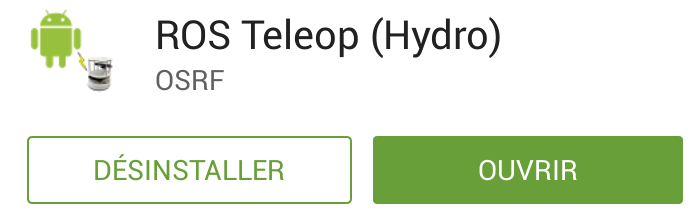
\includegraphics[width=0.5\textwidth]{images/turtlebotTeleopApp.png}
\end{center}

Now your device is ready.

\subsubsection{Different bringup}

\begin{tabbing}
\hspace{1cm}\=\hspace{1cm}\=\kill
There are three different ways to bringup the turtlebot :\\\\

\> -The \textbf{Minimal}, which we used previously.\\\\



 And two others : \\
\> -The \textbf{App Manager}, which can do everything minimal does, but also offers the option \\ of managing your programs as robot apps via the app manager.\\\\

\> -And the \textbf{Android Enabled}, which starts private/public masters and allows the app \\ manager to be controlled by a remote android device via the public master.\\\\
\end{tabbing}

\subsubsection{Concert}

What will be used for controlling with Android is the following statement : 
\begin{lstlisting}[frame=single]
$ rocon_launch turtlebot_bringup bringup.concert
\end{lstlisting}


 The concert is a multimaster framework running on top of the interactions and \textbf{rocon\_launch} is a multimaster version of roslaunch.\\
 
These ones allow us to launch the last two bringup launch files.
This is exactly what contains the \textbf{bringup.concert} : 
\begin{lstlisting}[frame=single]
<concert>
    <launch package="turtlebot_bringup" name="paired_public.launch" port="11311"/>
    <launch package="turtlebot_bringup" name="minimal_with_appmanager.launch" port="11312"/>
</concert>
\end{lstlisting}

It launches two linux shells (gnome-terminal or konsole) which spawn the following ros master environments : 

\begin{center}
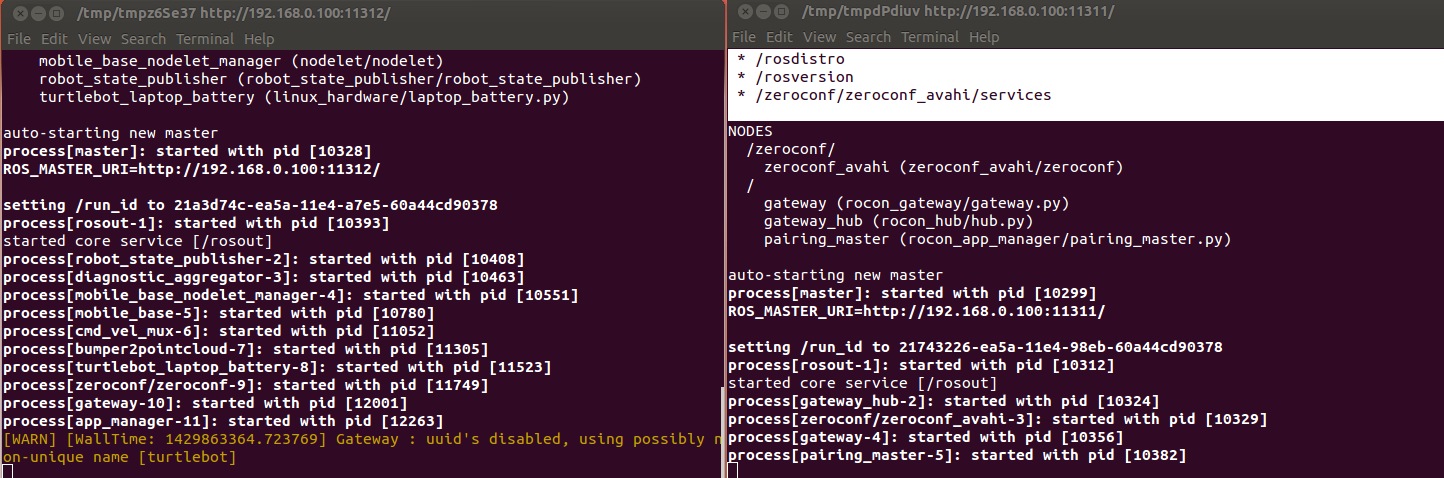
\includegraphics[scale=0.4]{images/twoMasters.png}
\end{center}

One is the \textbf{Private Master} : \\
\textbf{-Port:} 11312 \\
\textbf{-Software:} This master runs just the rocon gateway and robot app\_manager with a few default software, this means complex navigation as SLAM is not possible in this linux shell.\\

The other is the \textbf{Public Master} : \\
\textbf{-Port:} 11311 \\
\textbf{-Software:} This master runs another rocon gateway and a simple pairing script that assists the invitation of the private app\_manager and flipping the appropriate topics back and forth between the two masters. This one will be accessed by the android application.

In the application, you need to enter the public master, so you need to write the following URI to find the turtlebot : 
\begin{lstlisting}[frame=single]
http://192.168.0.100:11311/ 
\end{lstlisting}

\textbf{Here is the video of the result : }\\
\fbox{\url{https://www.youtube.com/watch?v=pBYmtod4o18}}
 
\subsubsection{Conclusion}

\end{document}